
\documentclass[tikz=false]{standalone}
\usepackage[utf8]{inputenc}
\usepackage[dvipsnames,svgnames]{xcolor}
\usepackage{tikz}
\usetikzlibrary{shapes.geometric}

\usetikzlibrary{positioning,graphs}


\begin{document}

  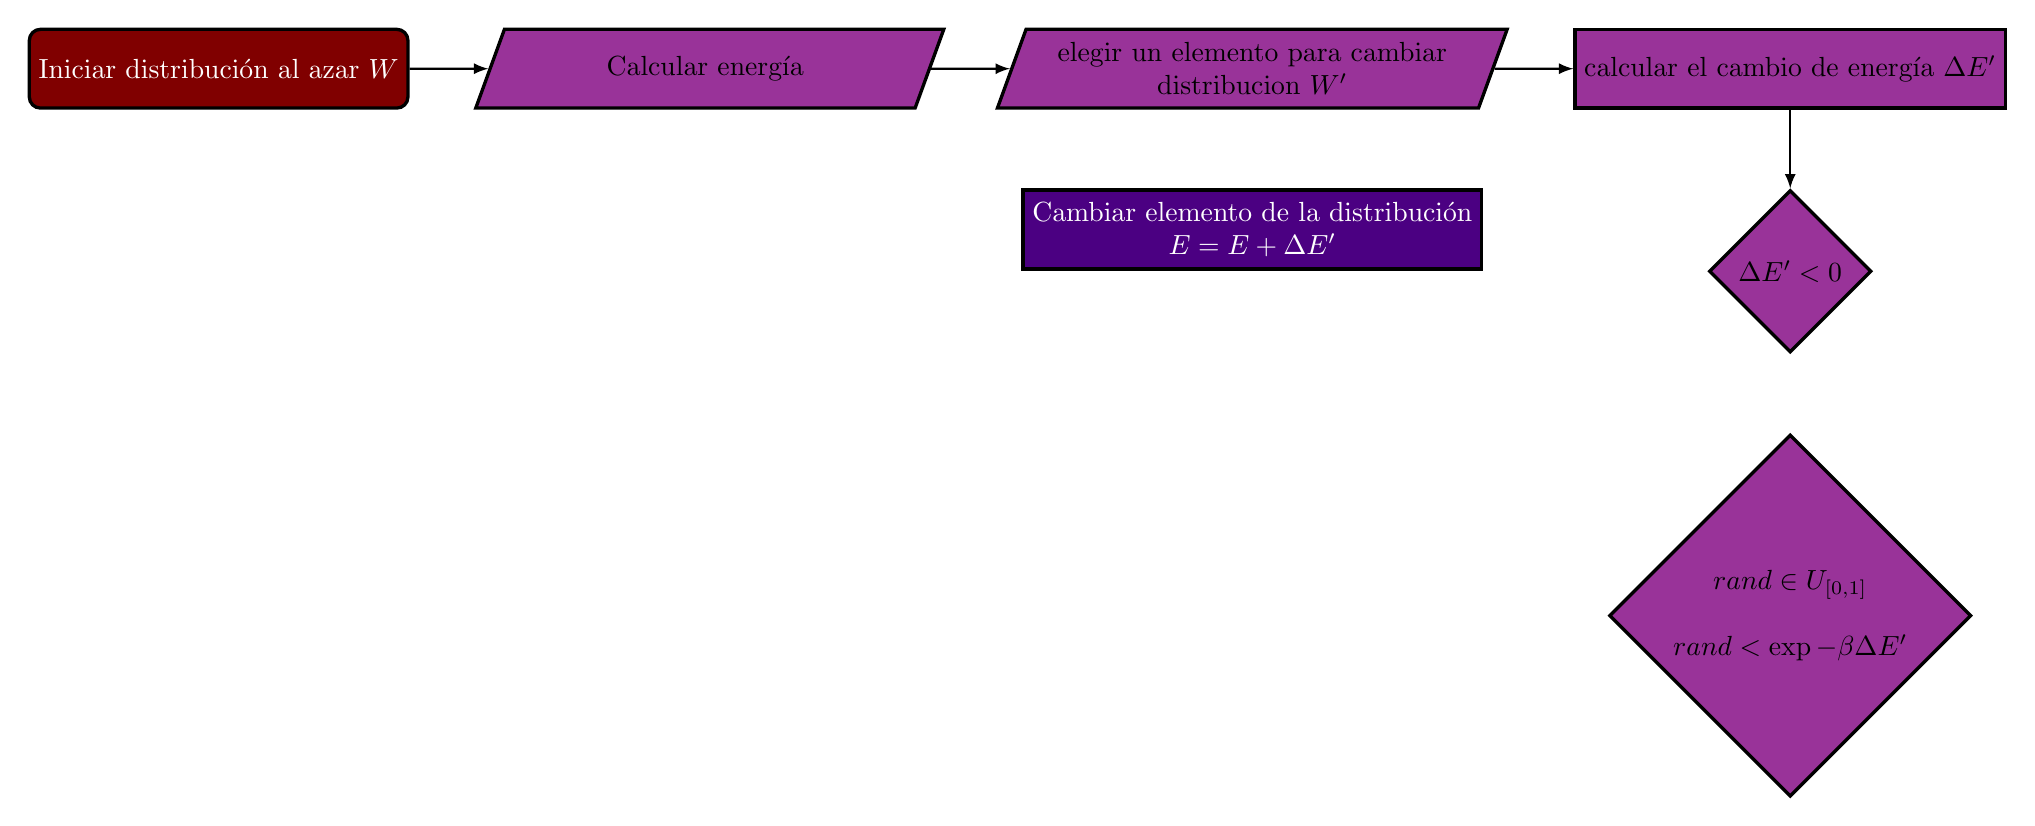
\begin{tikzpicture} [ node distance=1cm,>=latex,auto,
    every node/.style={rectangle, minimum size=1cm, draw, 
    fill=violet!80!white,very thick,align=center} ,
    astep/.style= {trapezium, trapezium left angle=70, trapezium right angle=110},
    start/.style= {rectangle, fill=Maroon, rounded corners,
    text = white},
    con/.style={->=stealth,thick },
    decide/.style={diamond,aspect=1},
    action/.style={rectangle, fill=Indigo, text=white}
    ]
    \node (n1) [start] { Iniciar distribución al azar $W$};
    \node (n2) [astep, right=of n1] { Calcular energía };
    \node (n3) [astep, right=of n2 ] { elegir un elemento para cambiar\\
                                            distribucion $W '$ };
    \node (n4) [ right=of n3 ] 
     {calcular el cambio de energía $\Delta E ' $};
        \node (n5) [decide, below =of n4 ] {$\Delta E' < 0 $};
        \node (n6) [decide, below =of n5 ]  
         { $ rand \in U_{[0,1]}$ \\ \\
	   $rand < \exp{-\beta \Delta E'} $};
    \node (n7) [below left= of n5, above left= of n6, below = of n3, action ]
    { Cambiar elemento de la distribución \\ $E = E + \Delta E'$ };

     \draw   [con]  (n1) -- (n2);
     \draw   [con]  (n2) -- (n3);
     \draw   [con]  (n3) -- (n4);
     \draw   [con]  (n4) -- (n5);
  \end{tikzpicture}

\end{document}
